\documentclass{report}
% pre\'ambuloasdf

\usepackage{lmodern}
\usepackage[T1]{fontenc}
\usepackage[10pt]{moresize}
\usepackage{amsmath} 
%\usepackage{fontspec}
%\setmainfont{Times New Roman}
\usepackage[spanish,activeacute]{babel}
\usepackage{mathtools}
\usepackage{graphicx}
\usepackage{subfig}
%\usepackage{anysize} 
\usepackage[%
    left=1.2in,%
    right=1.2in,%
    top=1.7in,%
    bottom=1.5in,%
    paperheight=11in,%
    paperwidth=8.5in%
]{geometry}

\title{TFG}
\author{Jorge Vela Pe�a}

\begin{document}
% cuerpo del documento


\large
%\marginsize{3cm}{2cm}{2cm}{2cm} 

%\rmfamily

\chapter{Despegue, busqueda y aterrizaje.}
\hspace{1cm} A lo largo de este cap\'itulo voy a contar las distintas fases por las que se ha pasado hasta llegar al algoritmo final. Se va a poder ver como se han producido diversos cambios a lo largo del proyecto. Esto se debe a que debido a las pruebas que se iban realizando, veiamos los fallos e imperfecciones y tratabamos de arreglarlos. Ademas, seg\'un el punto en el que nos encontraramos nos interesaba mas fijarnos en unos u otros detalles, por lo que no solo habia cambios en la base del algoritmo principal sino tambi\'en en el GUI(Interfaz Grafica de Usuario). Para la explicaci\'on de esto, abordar\'e el tema por partes. En primer lugar se har\'a una explicaci\'on del dise�o del algoritmo. Tras esto se explicaran las partes principales que tiene el procesado de la informaci\'on(percepci\'on, control, estados) para finalmente terminar explicando como ser\'ia una realizaci\'on completa del conjunto.

\section{Dise�o.}
\hspace{1cm} El dise�o de este algoritmo se trata de un ciclo continuo. Se trata de un proceso basado en adquisici\'on-procesado-envio de datos.La parte de adquisici\'on se realizar\'a gracias a los sensores del dron, los cuales obtendran cierta informaci\'on. Esta informaci\'on ser\'a transmitida al dispositivo que la procese, y una vez hecho esto el dispositivo enviara instrucciones al dron, que seran las que indiquen la velocidad,direcci\'on y sentido en el que este se tiene que desplazar.  Tenemos los sensores del dron, de los cuales la camara es el mas importante para este trabajo. Lo primero que hace el algoritmo, siendo esto la parte de adquisici\'on, es obtener la imagen. Dependiendo del punto del algoritmo en el que se encuentre, querra obtener una u otra informaci\'on de la imagen,pudiendo clasificar esta parte como procesado de la informaci\'on, para lo que siempre utiliza un filtro de color. Pongamonos en el caso de que el dron esta buscando una baliza en la que aterrizar(cuadrado que consta de dos colores), filtrara estos dos colores en la imagen obteniendo as\'i los objetos de interes. En caso de ver que hay un objeto que posiblemente sea la baliza, se eliminaran los objetos que sean menores a un determinado area, para asi evitar posible ruido que se haya introducido en la imagen u objetos que sabemos que no son los que buscamos. Tras esto el algoritmo realizara las operaciones que seran explicadas mas adelante para asegurarse de que se trata de una baliza.Llegando en este punto al envio de datos. En caso de tratarse de una baliza, el algoritmo enviara las instrucciones correspondientes, indicandole los movimientos a realizar comportarse frente a esta. En caso contrario, el algoritmo enviara las instrucciones para que continue con la busqueda. 


\section{Percepci\'on.}
\hspace{1cm} En este apartado se tratar\'a sobre el procesamiento de la imagen obtenida. Este puede ser el punto mas importante de todos, pues es gracias al cual el dron sabe en que punto del algoritmo se encuentra y que informaci\'on enviar. Las primeras pruebas no eran muy complejas, obteniamos una imagen RGB que era la que se transmitia, la convertiamos a HSV para que fuera mas facil su interpretaci\'on, debido a que no tenemos tres colores a los que tratar sino tres parametros( Matiz, saturac\'on y valor). Lo que se conseguia con esto era que un color no dependiera tanto de las condiciones del medio, pues variando poco los valores H y S no hay una gran modificaci\'on en el tono, y por lo tanto la intensidad de la luz influir\'a de menor manera. Tras esto se realiza un filtro de color, eligiendo los valores de H,S y V entre 0 y 255, quedandonos solo con los objetos que nos interesaban. Una vez estabamos en este punto, si se trataba de una imagen perfecta, como pueden ser algunas de simulador no hab\'ia problemas, pero en caso contrario, debido a factores como luces, sombras y reflejos, un color podia tratarse de distinta forma seg\'un el momento o que pasaran el filtro puntos de la imagen que no eran de las caracter\'isticas deseadas. Por ello,  era necesario el uso de operadores morfol\'ogicos, los cuales explico brevemente para que as\'i se entienda su uso: 
\begin{itemize}
	\item \textbf{Erosi\'on:} Dada una imagen y un elemento estructural, la erosi\'on es el conjunto de los elementos \textit{x} para los cuales el elemento estructural trasladado por \textit{x} est\'a contenido en la imagen. 
	\newline\hspace{1 cm} Aplicaci\'on: Cuando un pixel que parece pasar el filtro, pero los elementos de su alrededor(en concordancia con el elemento estructurante) no lo pasan, este pasa a ser parte del fondo. 
	\item \textbf{Dilataci\'on:} Transformaci\'on dual a la erosi\'on. El resultado de esta es el conjunto de elementos tal que al menos alg\'un elemento del conjunto estructurante esta contenido en \textit{x}, cuando el elemento estructurante se desplaza sobre \textit{x}
	\newline\hspace{1 cm} Aplicaci\'on: Pixeles que parecen de fondo, pasan a ser de la figura si estan cerca de pixeles que pasan el filtro.
	\item \textbf{Cierre:} Se trata de realizar una dilataci\'on en la imagen seguida de una erosi\'on.
	\item \textbf{Apertura:} Se trata de realizar la erosi\'on en una imagen seguido de la dilataci\'on.
\end{itemize}

\hspace{1cm} Pues bien, gracias a esto se puede hacer un pre-procesado de la imagen(t\'ecnica mediante la cual se mejoran y realzan las caracteristicas de esta para as\'i facilitar las posteriores operaciones a realizar) y asi obtener una mejor imagen con la qe trabajar. Hay que destacar que las mas utilizadas durante la realizaci\'on de este trabajo han sido la erosion y la apertura. Pues con la erosi\'on evitabamos que se colaran pixeles de fondo como parte del objeto, por lo que obteniamos solo la parte requerida, y por otro lado con la dilataci\'on realizada en la apertura, tras eliminar el ruido de fondo, si en alg\'un objeto se quedaba un pixel en negro conseguiamos que este pasara a formar parte de la figura, por lo que con estos metodos habiamos conseguido el objetivo: eliminar el ruido de fondo y obtener el objeto de forma mas compacta.En la siguiente imagen podemos observar un ejemplo de esto:

\begin{figure}[ht]
	\centering
		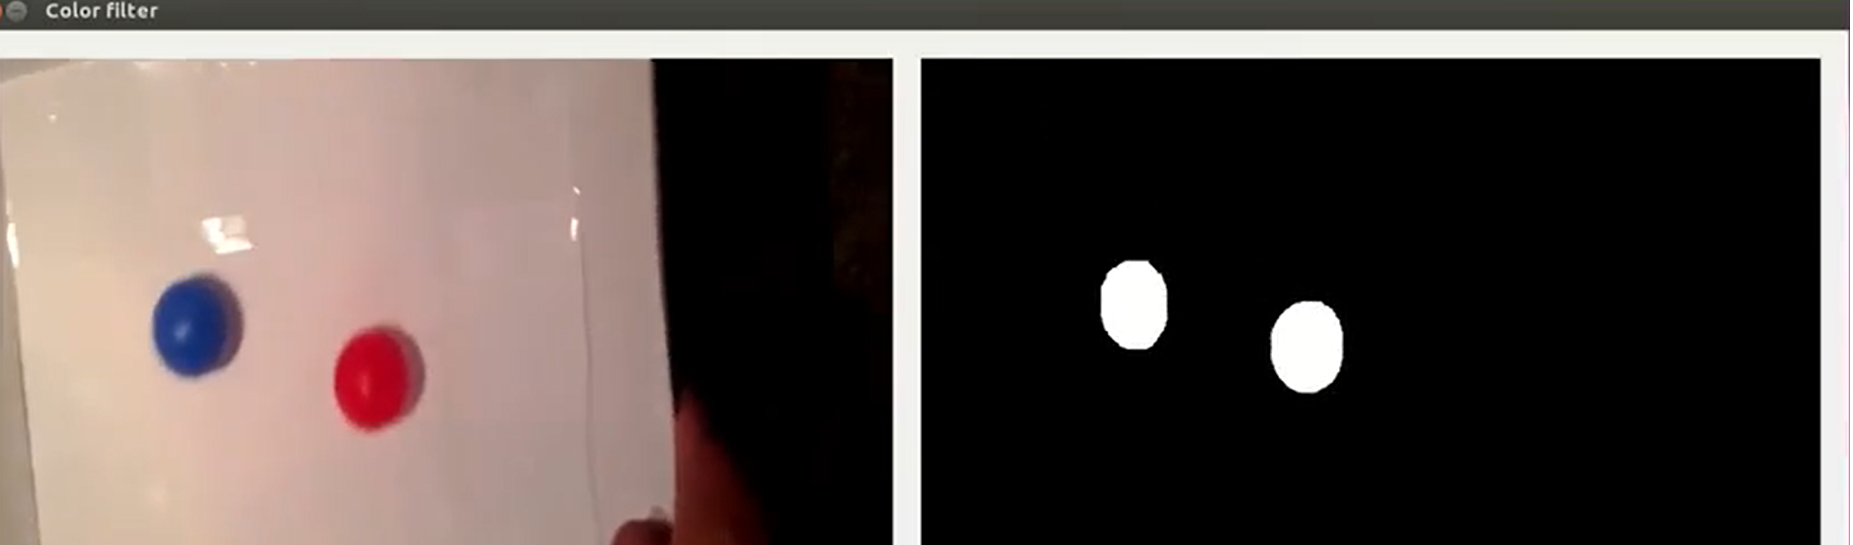
\includegraphics[width=1.0\textwidth]{imgs/colorfilter.eps}
		\caption{Esta imagen muestra un primer filtro de color.}
	\label{fig:ColorFilter}
\end{figure}

\hspace{1cm} A continuaci\'on pongo como ejemplo una parte de codigo, el cual coge una imagen, la convierte a HSV, crea un filtro de color y pasa la imagen a traves de este, obteniendo una imagen resultante:
\begin{verbatim}
hsv = cv2.cvtColor(input_image, cv2.COLOR_BGR2HSV)
lower_orange = np.array([100,100,80], dtype=np.uint8)
upper_orange = np.array([150, 255,255], dtype=np.uint8)
maskOrange = cv2.inRange(hsv, lower_orange, upper_orange)
maskRGBOrange = cv2.bitwise_and(input_image,input_image, mask= maskOrange)
\end{verbatim}
\hspace{1 cm} Destacar que con la \'ultima linea de este codigo, conseguiriamos que la imagen resultante no quedara en blanco y negro, sino que lo objetos que pasan el filtro se mostraran en su color original. 

\hspace{1 cm} Con esto se obtuvo una primera buena se�al, y era que sobre imagenes reales(con imperfecciones) conseguiamos realizar los filtros que queriamos, por lo que el siguiente paso fue decidir la forma que tendr\'ia la baliza y comenzar a trabajar en ella y sus caracter\'isticas. Esta baliza constaria de un cuadrado formado por 4 cuadrados de dos colores: 

\begin{figure}[ht]
	\centering
		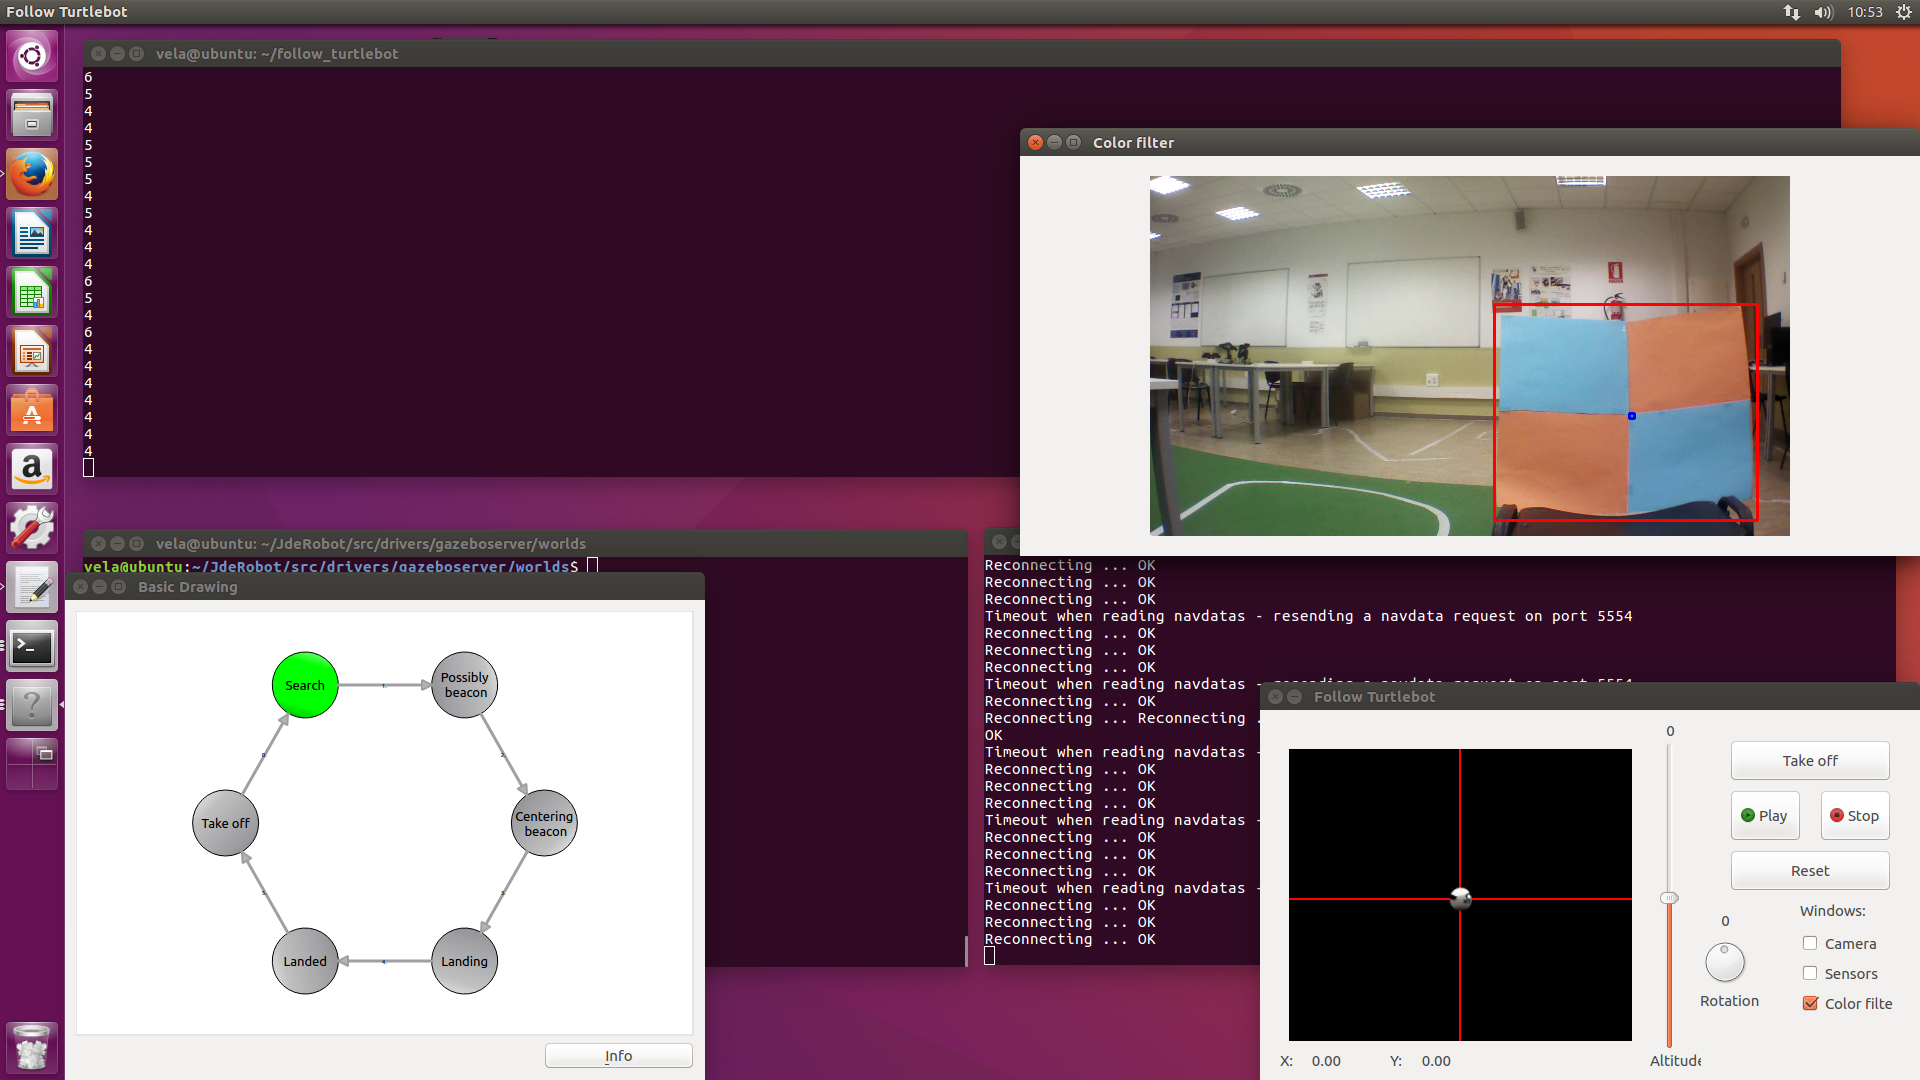
\includegraphics[width=0.4\textwidth]{imgs/k_beacon2.eps}
		\caption{Esta imagen muestra el conjunto de herramientas utilizadas.}
	\label{fig:Herramientas}
\end{figure}

\hspace{1 cm} Con la imagen de simulador, lo que tuvimos que hacer fue cambiar los valores al filtro de color anterior, con lo que ya conseguiamos obtener los colores de la baliza, pero sobre la baliza real se estuvo mas tiempo trabajando, pues al trabajar con ella en distintos entornos hab\'ia muchos cambios de luminosidad, y aunque HSV minimizara este problema, seg\'un el entorno de trabajo segu\'ia dando problemas. Al final ampliando el rango de colores, un mejor pre-procesado de esta imagen y el procesado para el algoritmo, se consigui\'o que esto no fuera un problema. 

\hspace{1 cm} Pero en realidad en este punto solo teniamos el primer paso, que la baliza pasara el filtro de color, ahora teniamos que conseguir que nuestro algoritmo detectara eso como una baliza para poder posicionarse sobre ella. Para este punto, se ha pasado por distintos puntos y algoritmos, los cuales se han ido mejorando o cambiando seg\'un los fallos que se veian, hasta llegar a un algoritmo final.

\hspace{1 cm} Lo primero que hicimos fue sobre el simulador. Se obtenia la posici\'on de los pixeles donde se encontraba el objeto que pasaba el filtro, y a partir de esto se calculaba su pixel central. Esto se hacia gracias a una funci\'on de OpenCV que retornaba el area que no se consideraba fondo, y luego de este area calculaba su centro. Un ejemplo del codigo python que realiza esto, a partir del codigo anterior, es el siguiente:

\begin{verbatim}
momentsOrange = cv2.moments(maskOrange)
x_center = int(momentsTot['m10']/momentsTot['m00'])
y_center = int(momentsTot['m01']/momentsTot['m00'])
\end{verbatim}

\hspace{1cm} Una vez hemos obtenido el centro del objeto, hay que calcular el centro de la imagen. En este caso, para calcularlo, hemos hecho es que la primera vez que se ejecute nuestro algoritmo(teniendo en cuenta que este est\'a en una continua ejecuci\'on) llame a una funci\'on a la que se le pasa la imagen de entrada, obtiene su tama�o y calcule a partir de este cual es el centro de la imagen. La raz\'on de hacer esto es que tanto el dron real como el del simulador tienen dos camaras, que obtienen distintas imagenes con distintos tama�os, de esta forma se calcula el tama�o la imagen que se va a utilizar de manera autom\'atica antes de comenzar cualquier proceso. Pues bien, para hacer las pruebas iniciales, teniendo el centro de la imagen y el centro del punto al que queremos llegar, basta con hacer la resta de estos y multiplicarlos por un valor(en funci\'on de las velocidades del dron) para que este se mueva, centrando su centro y el del objeto. 

\hspace{1cm} Tras conseguir, con un filtro y unas funciones, que el dron pudiera situarse sobre un objeto fitrado, pasamos a mejorar la detecci\'on de la baliza. La idea principal de la detecci\'on es detectar donde esta la cruz que forman los 4 cuadrados de colores, o lo que es lo mismo, detectar la intersecci\'on de los cuadrados de la baliza, as\'i obtendremos el punto sobre el cual situarnos para podernos centrar. 

\hspace{1cm} Un primer algoritmo fue realizar los dos filtros de color, uno por cada color de la baliza, obteniendo as\'i por separado los colores verde y naranja cuando trabajabamos en el simulador. Una vez obteniamos las imagenes por separado realizamos una dilataci\'on de ambas im\'agenes y luego una suma, lo que nos daba como resultado otra vez la baliza inicial pero con las intersecciones de otro color, de forma que filtrando por este nuevo color obtenido obteniamos la cruceta de la baliza. En este punto en el \textit{color filter} de la herramienta veiamos los dos filtros por separado y la intersecci\'on de ambos:

\begin{figure}[ht]
	\centering
		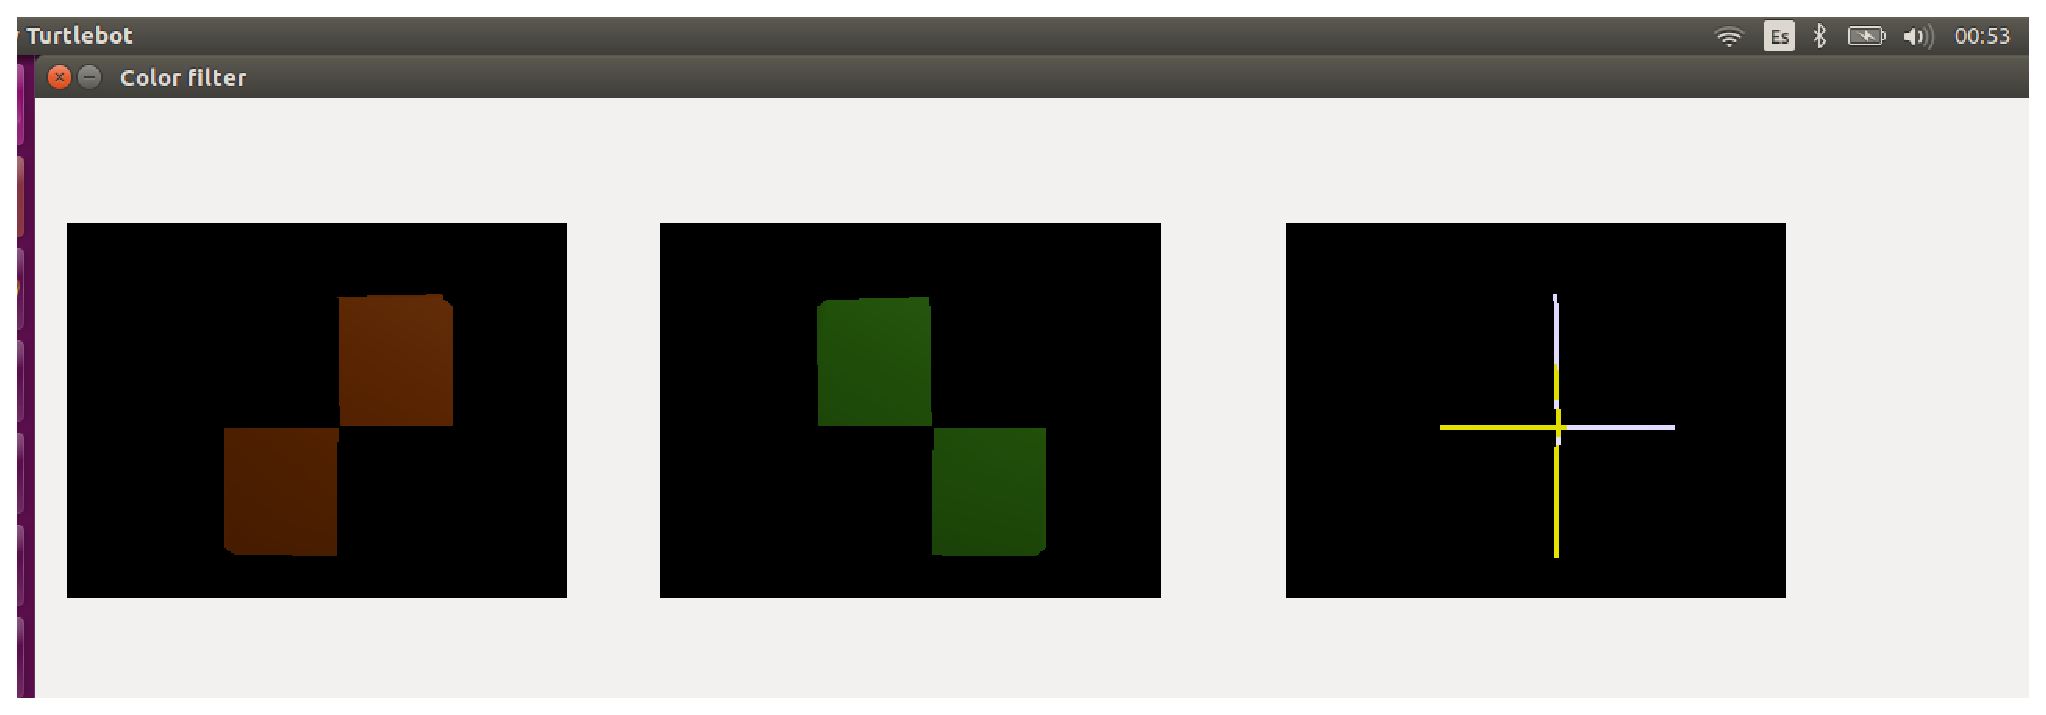
\includegraphics[width=0.8\textwidth]{imgs/E_Imagen_baliza.eps}
	\label{fig:E_Imagen_baliza}
\end{figure}

\hspace{1cm} En este punto, cuando el dron detectaba un objeto en la figura de la izquierda, lo trataba como baliza, por tener los dos colores principales juntos, pero aun quedaba mucho camino por recorrer, pues no detectabamosel centro de la intersecci\'on. Por otro lado, fue en este punto donde decidimos que las ventanas que mostraba el \textit{color filter} ya no era tan necesaria, pues habiamos obtenido lo que queriamos, y se decidi\'o trabajar hacia una ventana que mostrara la imagen completa de lo que estaba viendo el dron y marcara de alguna forma el contorno y cruceta de dicha baliza. Para esto fueron muy utiles las funciones \textit{findContours} y \textit{drawcontours} de OpenCV, las cuales nos permitian encontrar los bordes de los objetos de las imagenes y marcar estos. Lo que haciamos en este proceso era obtener los bordes de las imagenes que hab\'ian pasado el filtro y despues pintar sobre la imagen original.Para poder utilizar esta funci\'on necesitabamos pasar la imagen a escala de grises, como podemos ver a continuaci\'on:

\begin{verbatim}
imgray1 = cv2.cvtColor(maskRGBOrange,cv2.COLOR_BGR2GRAY)
ret,thresh = cv2.threshold(imgray1,255,255,255)
_,contours, hierarchy = cv2.findContours(thresh,cv2.RETR_TREE,cv2.CHAIN_APPROX_SIMPLE)
cv2.drawContours(input_image, contours, -1, (0,255,0), 5)
\end{verbatim}

\hspace{1cm}Conseguido esto, para el simulador teniamos un algoritmo principal que hac\'ia lo que buscabamos en situaciones ideales, pero seguia teniendo varios fallos.
\hspace{1cm} El primero a arreglar era que si en lugar de 4 cuadrados la baliza solo tenia dos, al dilatar y filtrar obtendriamos de igual forma otra figura, aunque en lugar de una cruceta se tratara de una linea. La forma de enfrentarse a esto fue contando el numero de objetos que hab\'ia en la imagen. Si la imagen ten\'ia dos objetos de cada color y un objeto que fuera la intersecci\'on de los otros, se trataria de una baliza, en caso de no ser de esta forma no se trataria como tal. En la parte de visi\'on estuvimos mucho tiempo trabajando con este algoritmo, pues para el simulador funcionaba bien. Pero en este punto, en la parte de visi\'on, detecci\'on de colores y realizaci\'on del filto, comenzamos a trabajar con el dron real, haciendo tareas muy simples, por lo que mejorar la robustez de esto se quedo un poco de lado. 

\hspace{1cm} Para comenzar a probar el filtro de colores en el dron real se hizo una baliza como la que teniamos en el simulador, pero al ir a realizar las primeras pruebas estaba el problema de que en la realidad hab\'ia muchos colores parecidos en las distintas direcciones, por lo tanto el dron confundia muy facil los colores. Para arreglar esto se empezo trabajando sobre un color y mejorando el algoritmo, de tal manera que el rango de colores fuera mas reducido, y aunque esto era un problema porque al trabajar con la luz real, un mismo color variaba mucho su rango segun la situaci\'on que estuviera, trabajando en HSV se consiguio, y tras esto en el pre-procesado se realiz\'o una erosi\'on con mas iteraciones de forma que eliminaba mejor los pixeles de fondo, pues en estas pruebas el problema era que uno de los colores de fondo era muy parecido al color de la cartulina. Tambi\'en a�adimos que el dron solo hiciera caso a los objetos con un area mayor a determinado valor, con lo que conseguiamos que si alg\'un objeto de fondo segu\'ia pasando el filtro lo obviara.

\hspace{1cm} Despues de esto ya quedaba la ultima parte por parte del filtro de colores aunque la mas dificil: \textit{conseguir situar una baliza en condiciones reales}. La primera complicacion de esto es el detectar dos colores muy distintos, el problema de esto era que en cualquier entorno que estuvieramos era muy probable tener de fondo un color muy parecido a cualquiera de los dos, pero como anteriormente, fue reforzar el filtro y pre-procesado para conseguir esto. Una vez conseguimos las pruebas eran sencillas: hacer despegar al dron y poner la baliza delante. Una vez que movieramos la baliza el dron deb\'ia moverse en el mismo sentido, prueba que, aunque costosa, se realizo con exito. Destacar que tambi\'en en este momento la imagen que mostraba \textit{color filter} se volvio a modificar, pues se mostraba la imagen real y sobre ella se pintaba, si era posible baliza, los bordes y la cruceta en verde. En el momento que se trataba de la baliza real, los bordes se pintaban en rojo (valor RGB 255,0,0) y la cruceta en verde (valor RGB 0,255,0). De esta forma era muy facil saber, con solo visualizar la imagen, en que punto se encontraba el algoritmo y si actuaba correctamente.


\hspace{1cm} Ya con un algoritmo de detecci\'on con el que se pod\'ia trabajar correctamente, todav\'ia le faltaba algo de robustez, pues si situabamos un objeto del mismo color que alguno de los colres de la baliza lo detectaba como un objeto mas, lo que llevaba a que el numero de objetos de un color fuera mayor, y daba problemas como el que el n\'umero de objetos de un color fuera mayor, el area era mayor que el deseado y en caso de calcular el centro del area no lo situaba donde deb\'ia. Por lo tanto, se llego a una soluci\'on que, aunque tardaba mas en procesar la imagen, es mas robusta. El proceso es el siguiente:
\begin{enumerate}
	\item Como anteriormente, pasar los filtros de color y obtener solo los objetos de los colores deseados, pasando el resto a ser p\'ixeles de fondo. De aqui obtenemos dos im\'agenes, una por color.
	\item De cada imagen, obtenemos el n\'umero de objetos, sus areas y sus contornos. Vamos recorriendo los objetos de las imagenes,  en caso de tener un area mayor a un valor determinado, se crea una imagen negra del mismo tama�o que la imagen de entrada, y se pinta sobre esta el contorno del objeto con un valor determinado, ponamos como ejemplo que cada contorno tiene un valor RGB (0,1,0). De forma que, si por ejemplo, el numero de objetos tras pasar los dos filtros era 5, obtendremos 5 imagenes. 
	\item Por cada imagen obtenida, dilatamos lo obtenido(por lo que el borde se ensanchara) y lo sumamos a una imagen final, de forma que en cada imagen, donde se situe el contorno se sumara a cada pixel un valor RGB(0,1,0). De forma que el punto que sea la intersecci\'on de dos objetos, el valor sera(0,2,0) y donde sea la intersecci\'on de 4 objetos el valor sera (0,4,0). El punto donde interseccionen 4 objetos ser\'a la cruceta (ejemplo de la suma de imagenes en figura 4).
	\item Una vez tenemos esta im\'agen final, le podemos aplicar un filtro RGB que permita pasar los p\'ixeles con valor (0,4,0), de forma que de la cruceta solo obtendremos el punto donde interseccionan los 4 cuadrados.
	\item Ya con la imagen que solo muestra los p\'ixeles de intersecci\'on, podemos utilizar la funci\'on drawcontours, que a parte de permitirnos marcar el centro sobre la imagen original, nos retorna el valor de los pixeles que pinta, de donde obteniendo su centro, podemos obtener con exactitud los valores X e Y donde se situa la cruceta.
	%\item Ya teniendo este valor, por otro lado hemos continuado con la realizaci\'on de otro filtro, el cual pinta de verde los bordes de los objetos sobre la imagen original, miramos si el valor (X,Y) obtenido en el filtro anterior coincide con un valor pintado en esta imagen. En caso de coincidir podemos asegurar que e trata del centro de la baliza.
	\item Para finalizar este proceso, se realizo de nuevo un cambio en \textit{color filter}, en el cual con la funcion rectangle de OpenCV marcamos la cruceta de la baliza(como se puede ver en la figura dos de la p\'agina 17) y con un cuadrado rojo los objetos que son posibles balizas, marcando de esta forma la baliza real.
\end{enumerate}
\vspace{2mm}
\begin{figure}[ht]
	\centering
		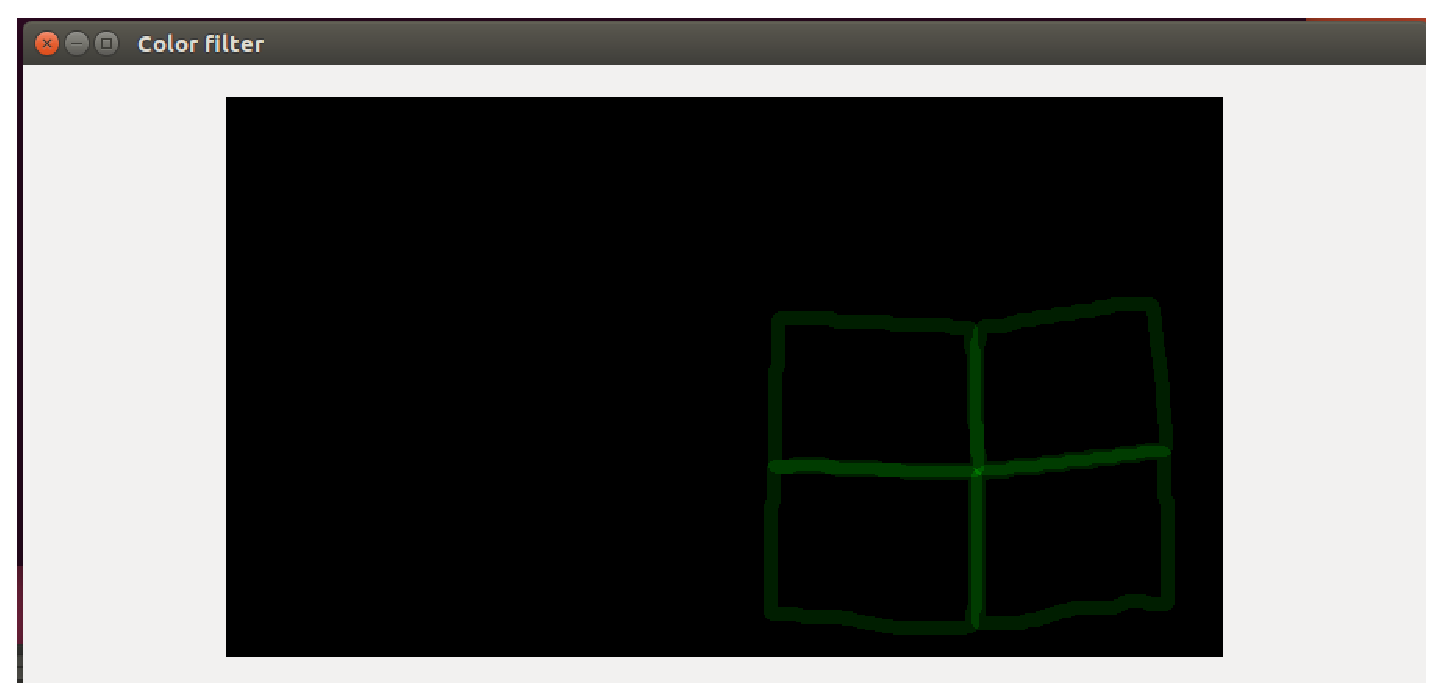
\includegraphics[width=1.1\textwidth]{imgs/k_Beacon1.eps}
		\caption{Imagen que muestra la suma de las diferentes imagenes creadas por cada objeto.}
	\label{fig:k_Beacon1}
\end{figure}
\vspace{3mm}

\hspace{1cm} A continuaci\'on inserto un fragmento de c\'odigo, el cual a partir de una imagen que ha pasado un filtro, pinta los contornos de cada objeto, cada uno sobre una nueva imagen negra, y las guarda en un array. Tras esto dilata y suma las imagenes obteniendo la imagen final.

\begin{verbatim}
f = []
i=0
imgray2 = cv2.cvtColor(maskRGBOrange,cv2.COLOR_BGR2GRAY)
ret,thresh = cv2.threshold(imgray2,255,255,255)
_,contours, hierarchy = cv2.findContours(thresh,cv2.RETR_TREE,cv2.CHAIN_APPROX_SIMPLE)
areas = [cv2.contourArea(c) for c in contours]
for extension in areas:
    if extension > 100:
    img = np.zeros((y_img*2,x_img*2,3), np.uint8)
        actual = contours[i]
        approx = cv2.approxPolyDP(actual,0.05*cv2.arcLength(actual,True),True)
        cv2.drawContours(img,[actual],0,(0,30,0),12)
        f.append(img)
        i=i+1
			
kernel = np.ones((3,3),np.uint8)
if(len(f)>0):
    f[0] = cv2.dilate(f[0],kernel,iterations = 4)
    show_image2=f[0]
    for k in range(len(f)-1):
        f[k+1] = cv2.dilate(f[k+1],kernel,iterations = 4)
        show_image2=show_image2+f[k+1]
		
\end{verbatim}

\hspace{1cm} Por otro lado, voy a mostrar un fragmento de c\'odigo en el cual, a partir de la imagen que muestra el borde de la baliza, la cruceta y el centro en determinados valores, obtengo los pixeles sobre los que se centra la cruceta. La raz\'on de que se inicien a un valor negativo es para que al retornar estos valores cuando se llama a la funci\'on, el algoritmo sepa que no se ha detectado la intersecci\'on entre los cuatro cuadrados de la baliza. 


\begin{verbatim}
lower_green = np.array([0,80,0], dtype=np.uint8) 
upper_green = np.array([0, 255,0], dtype=np.uint8) 
maskSHI = cv2.inRange(show_image2, lower_green, upper_green)
show_image2 = cv2.bitwise_and(show_image2,show_image2, mask= maskSHI)

compare_image = np.zeros((y_img*2,x_img*2,3), np.uint8)
diff_total = cv2.absdiff(compare_image, show_image2)

imagen_gris = cv2.cvtColor(diff_total, cv2.COLOR_BGR2GRAY)
_,contours,_ = cv2.findContours(imagen_gris,cv2.RETR_EXTERNAL,cv2.CHAIN_APPROX_SIMPLE)

positionX=-1
positionY=-1
for c in contours:
    if(cv2.contourArea(c) >= 0):
        posicion_x,posicion_y,ancho,alto = cv2.boundingRect(c) 
        cv2.rectangle(show_image,(posicion_x,posicion_y),(posicion_x+ancho,posicion_y+alto)
        ,(0,0,255),2)
        positionX= (posicion_x+posicion_x+ancho)/2
        positionY= (posicion_y+posicion_y+ancho)/2
\end{verbatim}

\section{Control.}
\hspace{1cm} Una vez terminado el filtro de color, hablemos del algoritmo de movimiento del dron. Las primeras pruebas sobre simulador se realizaban de forma simple: El dron despegaba, y mientras no detectara baliza sobre la que centrarse, subia dando vueltas sobre si mismo, en el momento que encontraba la baliza obten\'ia el centro de esta e intentaba que coincidiera con el centro de la imagen. Tras esto se probo que la baliza se desplazara y que el dron fuera capaz de seguirla. Prueba que tambi\'en funciono sin problemas. Al depender la velocidad de la resta de los centros, provocaba que al estar mas lejos la velocidad de movimiento fuera mayor y fuera disminuyendo conforme se centraba, evitando de esta forma que el dron frenara de forma brusca y disminuir los balanceos y turbulencias. 
Aun as\'i, se detectaban ciertas inperfecciones debido a que se trataba de un controlador proporcional, el cual funcionaba bien pero no lo suficiente, por lo que se decidio a�adir una componente derivativa, con el objetivo de mantener el error al minimo, evitando que este se incremente y por lo tanto el dron sufra cada vez mas oscilaciones al situarse sobre un punto. Este control se basa en derivar el error con respecto al tiempo y multiplicarlo por una constante. Dado que nuestro algoritmo ejecuta una vez cada cierto tiempo y no esta continuamente pasando por este punto, podemos considerar que se trata de un sistema en tiempo discreto, y por tanto en lugar de trabajar con derivadas trabajaremos con sumatorios. De esta forma, para a�adir un control deriavtivo realizabamos una operaci\'on que depende de la velocidad anterior y la que tenemos ahora: \[v_{derivativa} =1-(v_{anterior}-v_{nueva})/50 \]  
\hspace{1cm} En nuestro algoritmo, en caso de que la operaci\'on de un valor menor a 0.1 lo igualamos a este, con lo que conseguimos que nunca sea un valor muy cercano a 0 y por lo tanto no se quede en el sitio. Este resultado lo multiplicamos a la velocidad final, y lo que conseguimos es que si el valor entre dos velocidades continuas es muy alto este se aten\'ue de forma que el dron no cambie mucho y vaya oscilando, sino que lleve una velocidad mas continua, de cara a acelerar o frenar su velocidad. 

\hspace{1cm} Por otro lado, el dron tiene un algoritmo de busqueda, en el que se pretende que se mueva realizando una espiral continua, haciendo as\'i que recorra toda la zona de su alrededor. Para ello se le env\'ia la informaci\'on de dos velocidades que fueran variando con el paso de las iteraciones, una que depend\'ia de la rotaci\'on sobre si mismo, y otra velocidad que se le pasaba para que hiciera en su eje X hacia delante. De esta forma, con el paso de las iteraciones disminuia la velocidad de rotaci\'on, al mismo tiempo que aumentaba la velocidad hacia delante, con lo que conseguiamos un algoritmo de busqeda en espiral, pudiendo recorrer de esta forma un determinado area con facilidad. Un ejemplo de esto lo podemos ver en el siguiente fragmento de c\'odigo.

\begin{verbatim}
self.cmdvel.sendCMDVel(1.8+wSearch,0,0,0,0,1.5 - wSearch)
numVuelta=numVuelta+1
if(numVuelta==100):
    timerW=timerW+(timerW/8)
    numVuelta=0
    if(wSearch<1):
        wSearch=wSearch+0.2
\end{verbatim}

\hspace{1cm} Por ultimo, otra herramienta que se utilizo fue el diagrama de estados gracias a la herramienta visualStates. Esta parte es sencilla, al arrancar la aplicaci\'on se pueden crear distintos estados haciendo que unos apunten a otros, de tal forma que puedes ver el punto en el que se encuentra el algoritmo. Cada vez que pasas por una parte del c\'odigo, indica en que punto se encuentra y este se marca con color verde sobre el diagrama. En un principio este diagrama constaba de tres estados, despegue, busqueda y aterrizaje(que como veremos mas adelante, son las partes principales del algoritmo), aunque para tener mas datos modificamos para tener despegue, busqueda, posible baliza, centrandose sobre la baliza, aterrizando y aterrizado.	Este nos fue de gran utilidad, pues cuando en un inicio planteamos los posibles estados que hab\'ia y sus distintas transiciones vimos que hab\'ia multitud de posibilidades, dependiendo de que parte viera de la baliza, si solo veia un color y al final encontraba dos o simplemente era otro objeto que coincidia, si por alguna casualidad perdia la baliza y tenia que comenzar el algoritmo desde el principio, o si todo iba correctamente. Gracias a que se mostraba este diagrama, era todo mucho mas sencillo.

\hspace{1cm} Para poder a�adirlo lo unico que se tuvo que hacer es a�adir dos paquetes del GUI de JdeRobot, uno que permitia abrir otra ventana y otro que permitia a�adir estados y transiciones entre ellos. Para marcarlo, siendo el numero que aparece el numero del estado que queremos marcar, val\'ia con la siguiente linea de c\'odigo:

\begin{verbatim}
self.machine.setStateActive(2, True)
\end{verbatim}

Visualmente, durante la ejecuci\'on obteniamos esto:
\begin{figure}[ht]
	\centering
		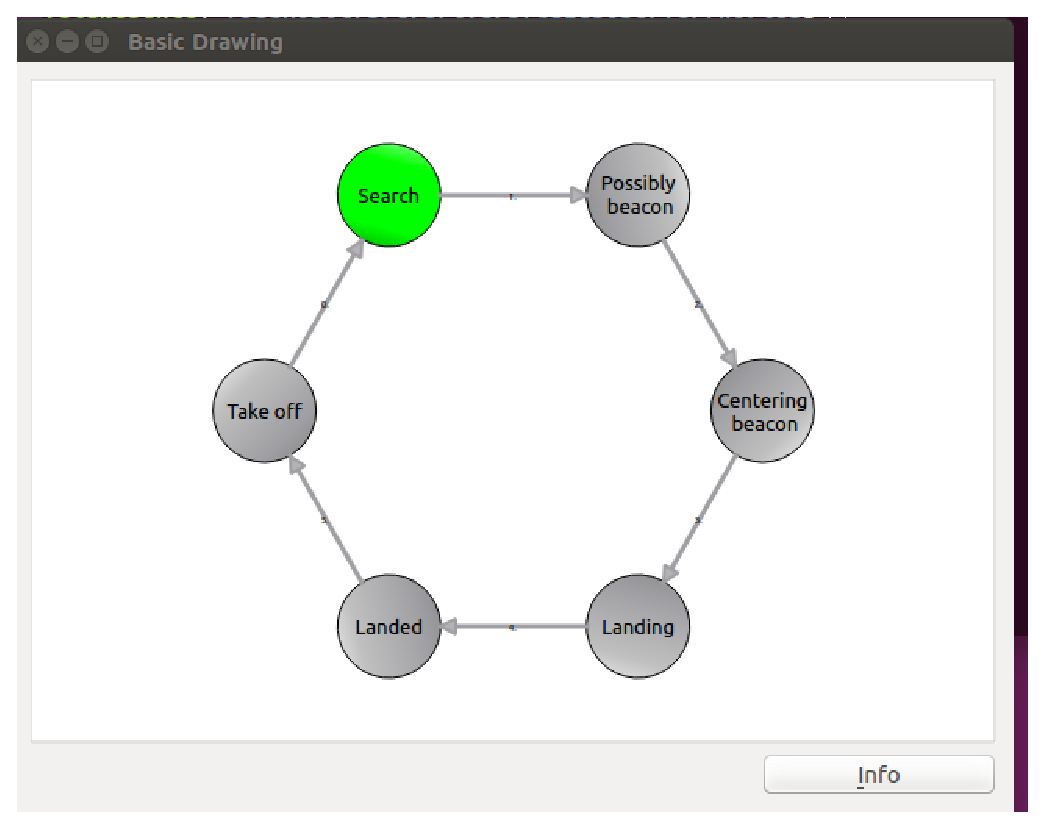
\includegraphics[width=0.3\textwidth]{imgs/states.eps}
		\caption{Imagen que muestra el diagrama de estados.}
	\label{fig:k_Beacon1}
\end{figure}

\section{Funcionamiento del algoritmo.}
\hspace{1cm} En realidad, todo lo contado del algoritmo sirve para satisfacer estas tres partes. 

\hspace{1cm} \textbf{El despegue} del dron. Para estas pruebas se ha estimado que el despegue constara de entre 5 y 10 segundos dependiendo el entorno en el que nos encontremos. Este varia principalmente por el espacio disponible, pues esta parte lo que pretende es levantarse del suelo y alcanzar cierta altura. Aunque es la parte mas sencilla, en un principio pensamos que todo ocurriria en perfecta forma, sin embargo al comenzar a trabajar con el ArDrone nos dimos cuenta de que bien por las corrientes internas que se forma en espacios cerrados, o por la inestabilidad de este simplemente por el paso del tiempo y que su estructura ya no esta en como en un inicio, una vez en el aire no mantenia la posici\'on, sino que se desplazaba cuando se le enviaban instrucciones de quedarse en el sitio(en mi caso,con el dron que trabajaba una vez se levantaba comenzaba a ir hacaia atras). Debido a esto, decidimos que el despegue se controlara tambi\'en mediante visi\'on. Lo que pretendiamos con esto es que una vez el dron estuviera en el aire, detectara una baliza de color naranja, calculara su centro e intentara situarse sobre este, asegurandonos as\'i realmente que el dron permanecia en el sitio. Trabajando en esta idea nos dimos cuenta que el dron ten\'ia un par de segundos en el despegue en los que trabajaba de forma autom\'atica y no es capaz de realizar las acciones que se le estan enviando, lo que lleva a estar los dos segundos iniciales sin control sobre este. Durante este periodo se marca el estado "`Take off"' en el diagrama de estados.

\hspace{1cm} Una vez tenemos el dron en el aire llegamos a la parte mas compleja, \textbf{la busqueda} de la baliza. En este momento se marca el estado "`Search"' en el diagrama de estados, y el dron comienza a moverse en forma de espiral mientras busca alg\'un objeto que tenga los colores de la baliza. En el momento que encuentra uno de los dos colores marca el estado "`Possibly beacon"' e intenta centrarse sobre el objeto, esperando que se trate de una baliza. En caso de no tratarse de la baliza, el dron se aparta de esta y continua con su algoritmo de busqueda, pero en caso de serlo marca sobre el diagrama de estados "`Centering beacon"' haciendo que coincidan sus centros. Aqui ya no se fija en el area del objeto como en el caso anterior, para centrarse sobre el centro de este, sino que al haber obtenido ya donde est\'a la cruceta, tiene sus valores desde un principio, por lo que es sobre estas coordenadas sobre las que tiene que situarse. Destacar que pueden darse factores externos por los cuales el dron pierda parte de la baliza y no la detecte como tal, pero si siga detectando objetos, en este caso tratara a tales objetos como la baliza e intentara situarse de nuevo sobre ellos durante un periodo de tiempo. En caso de tratarse de algun otro factor y que ya no exista baliza en este punto continuara buscando. Una vez el centro de la imagen y la cruceta estan a una distancia menor de un determinado n\'umero de p\'ixeles, aparte de centrarse comienza su descenso, hasta que la baliza en la imagen tiene un determinado area en el que se considera que ya esta suficientemente cerca y deja de descender. 

\hspace{1cm} Es en este momento cuando comienza la parte del \textbf{aterrizaje}, esto se debe a que el aterrizaje en si tambi\'en es un proceso que se realiza un poco a ciegas, pues en el momento que envias la instrucci\'on de "`land"' al dron este comienza a descender hasta que llega al suelo y para sus motores. Este momento se produce cuando el dron esta pr\'acticamente centrado sobre la baliza y a una distancia cercana, que nos podamos asegurar que en el periodo de aterrizaje no se va cruzar ningun obst\'aculo ni se van a producir accidentes. Se marca en el diagrama de estados "`Landing"' y el dron comienza a descender en vertical hasta encontrar el sitio donde posarse. Una vez aterrizado para sus motores y se marca el estado "`Landed"', habiendo finalizado de esta forma el algoritmo. 

\chapter{Experimentos.}
\hspace{1cm} Durante este cap\'itulo voy a contar las distintas pruebas que se han realizado durante todo el proceso. Cabe destacar que en un principio las pruebas fueron muy variadas y no todas se han utilizado en la idea final. Esto se debe a que en un principio teniamos diversas opciones e ideas, y fuimos investigando en ellas, pero por diversos factores no se llevaron a cabo. 

\hspace{1cm} En un principio la idea era hacer funcionar todo sobre el \textbf{3DR solo drone}, debido a sus muy buenas caracter\'isticas anteriormente explicadas. Para ello estuvimos, junto a otro compa�ero, un tiempo estudiando su funcionamiento y como podiamos acoplar este a la tecnolog\'ia JdeRobot. Fue un proceso costoso y donde pudimos detectar sus virtudes y defectos, pues tras probar el dron, manejandolo con su mando, veiamos que sus increibles caracter\'isticas como podian ser su potencia a la hora de los movimientos y la gran estabilidad que tenia al realizar movimientos bruscos con el. Tras esto, al comenzar a trabajar con las herramientas nos dimos cuenta del primer problema, el que levantaba la red WiFi no era el dron sino el mando que venia con el, el dron levantaba la red de radiofrecuencia y con esta se comunicaba por el mando, lo que conllevaba que la navegaci\'on del dron para ejecutar un algoritmo dependia de la distancia de este al mando. Buscando encontramos que la empresa estaba trabajando en una soluci\'on a esto, pero que tardar\'ia meses en llegar. Por otro lado se juntaba que el dron no ten\'ia una camara incorporada, ya que funcionaba con una GoPro, para la cual JdeRobot no tenia soporte. A todo esto habia que buscarle una soluci\'on, as\'i que se penso en a�adir una camara para la visi\'on de otra forma. Gracias a la potencia de este dron se le podian a�adir materiales sin que esto le impidiera volar, como era una \textit{intel compute stick} y una \textit{camara externa}. Realizamos pruebas con la intel computer stick y el ArDrone, el cual funcionaba sin problemas, y mas adelante probando la comunicacion de la intel con este drone levantando el servidor y por otro lado el ordenador comunicando con la intel y enviandole las instrucciones para que las realizara el dron, prueba que se realizo con exito. Al igual que funciono esto, tambi\'en funcionaron las pruebas con el dron 3DR Solo, pudiendo manejarlo con las herramientas JdeRobot y viendo sus datos cuando este realizaba movimientos. Tras esto, como la idea del algoritmo era que funcionara tambi\'en en interiores, por ejemplo en grandes naves industriales para el control y desplazamiento de mercancia, nos pusimos con esta prueba, lo que nos hizo darnos cuenta de que debido a su GPS, hasta que no encontraba una se�al lo suficientemente fuerte no te dejaba despegar, protocolo de seguridad por si habia alg\'un problema que pudiera utilizar su modo ``retunr home``. Pero utilizando el protocolo MAVLink desde el ordenador hab\'i un modo que te permitia evitar las restricciones de seguridad, haciendo asi que el dron despegara y pudiera ser utilizado en cualquier lugar. Fue al probar esto cuando la potencia del dron nos jug\'o una mala pasada, pues genero una cantidad de corrientes internas de aire que, en el momento de su despegue, en el cual hay unos segundos donde no se tiene control sobre el,no lo hiciera totalmente en vertical sino con una desviaci\'on hacia su izquierda, lo que llevo a chocar con distintos obst\'aculos. Por ultimo e intentando utilizar varios materiales juntos, probamos a unir la intel computer stick al ArDrone 2.0, para ver si ten\'ia suficiente fuerza como para volar con el, pero el ArDrone no consigui\'o levantarse del suelo. 

\hspace{1 cm} Tras la realizaci\'on de las pruebas y alguna mas que surgi\'o a raiz de estas, nos dimos cuenta de que habiamos obtenido grandes avances que sin haber realizado un trabajo conjunto podr\'ian habernos llevado mucho mas tiempo, pues esto nos aport\'o muchos datos que nos servirian mas tarde, a parte de aprender el funcionamiento de estos drones, los materiales que los componian y como realizar la comunicaci\'on dron-ordenador para el envio de informaci\'on y recibo de datos. Por todo esto y por los frentes que se iban abriendo para trabajar sobre el dron, fue cuando dividimos un poco mas nuestras tareas, ya no investigando un conjunto de cosas sino dividiendo las tareas y semanalmente poniendo en comun los avances que habiamos realizado, para ver que ibamos encaminados hacia el objetivo. En este punto fue cuando quedo marcada mi tarea principal para poder realizar este proyecto. \textbf{La detecci\'on de balizas y algoritmo de movimiento}. 

\hspace{1 cm} Ya se ha explicado antes como fue el desarrollo del algoritmo, pero la verdad es que las distintas pruebas realizadas son las que de verdad permitieron su desarrollo. 

\hspace{1 cm} Se comenzo trabajando con las camaras del ArDrone server en un espacio peque�o y cerrado, donde se consigi\'o un filtro para los dos colores de la baliza. Tras esto se quiso probar el dron en un espacio amplio,debido a que en espacios peque�os, al despegar el dron no se mantenia en el eje Z sino que lo hacia en diagonal, por lo que se chocaba con obstaculos como pod\'ian ser las mesas que hab\'ia, y ya se aprovech\'o para que asi pudiera realizar todo el algoritmo. Pero a la hora de detectar los colores se notaba la luz que entraba en todos los momentos y como iba oscureciendo con el atardecer, lo que llevo a que la prueba con el dron real no se hiciera sobre dos colores sino centrandonos solo en el naranja. Una vez consegido el filtro, el fondo del pabell\'on en el que estabamos, la pared era de un marron muy claro que se podia confundir con la baliza, por lo que se fijo mas la idea de obviar los elementos peque�os, y realizar una mayor erosi\'on, y entonces salio una primera prueba de gran valor, cuando nos situabamos delante del dron con la baliza , este aterrizaba:

\begin{figure}[ht]
 \centering
  \subfloat[Volando]{
   \label{f:volando}
    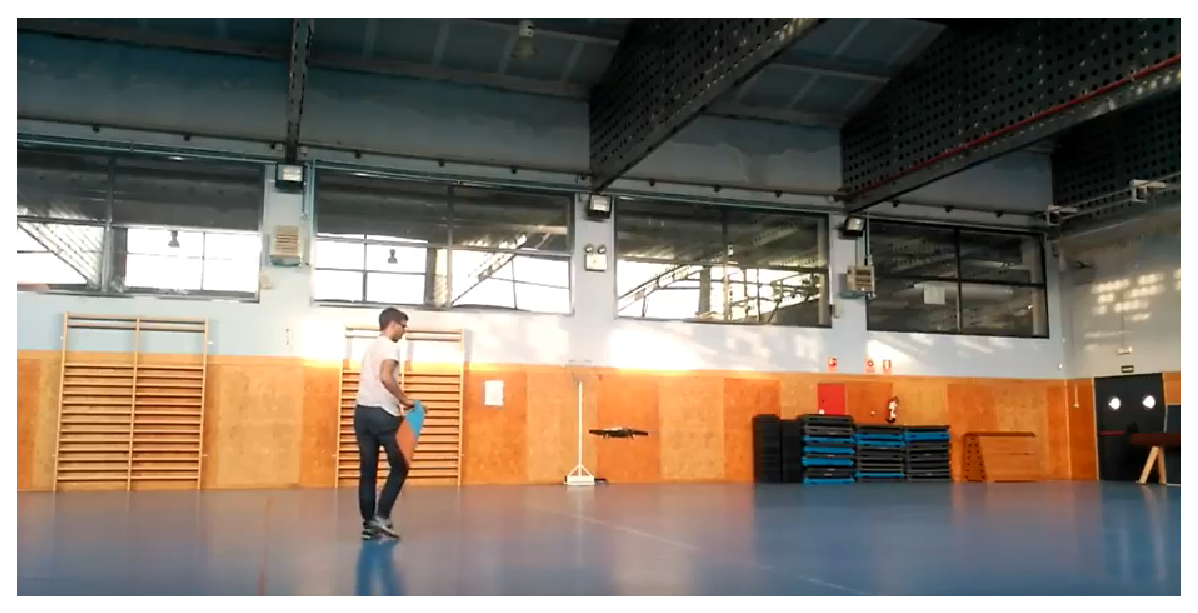
\includegraphics[width=0.3\textwidth]{imgs/balizaNaranja1.eps}}
  \subfloat[Aterrizando]{
   \label{f:aterrizando}
    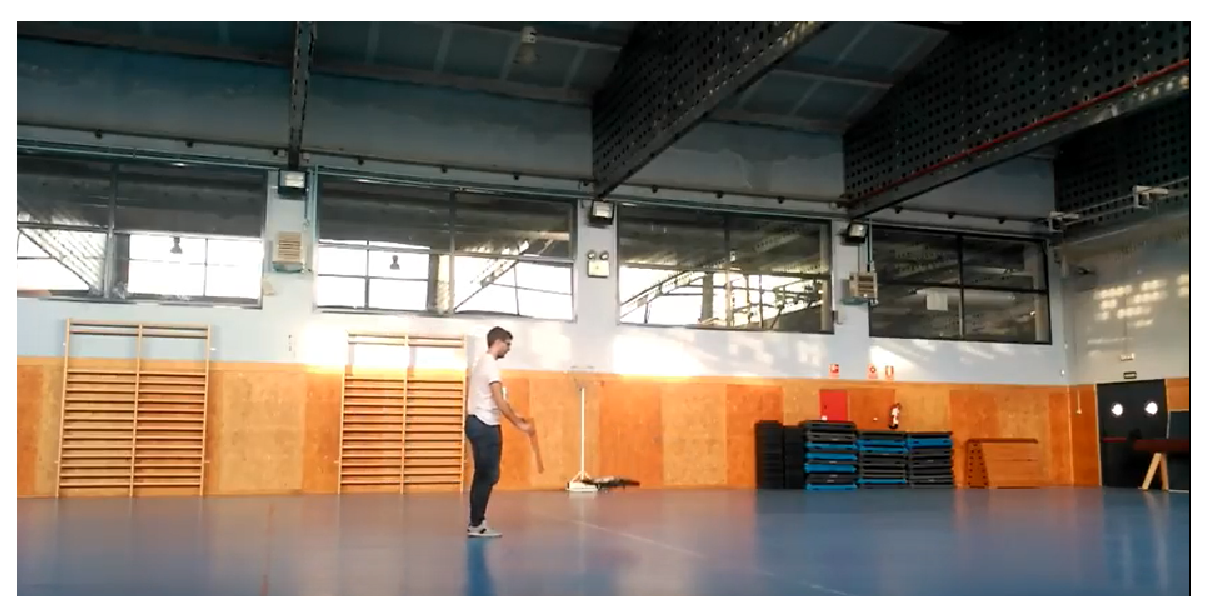
\includegraphics[width=0.3\textwidth]{imgs/balizaNaranja2.eps}}
  \subfloat[Aterrizado]{
   \newline\label{f:Aterrizado}
    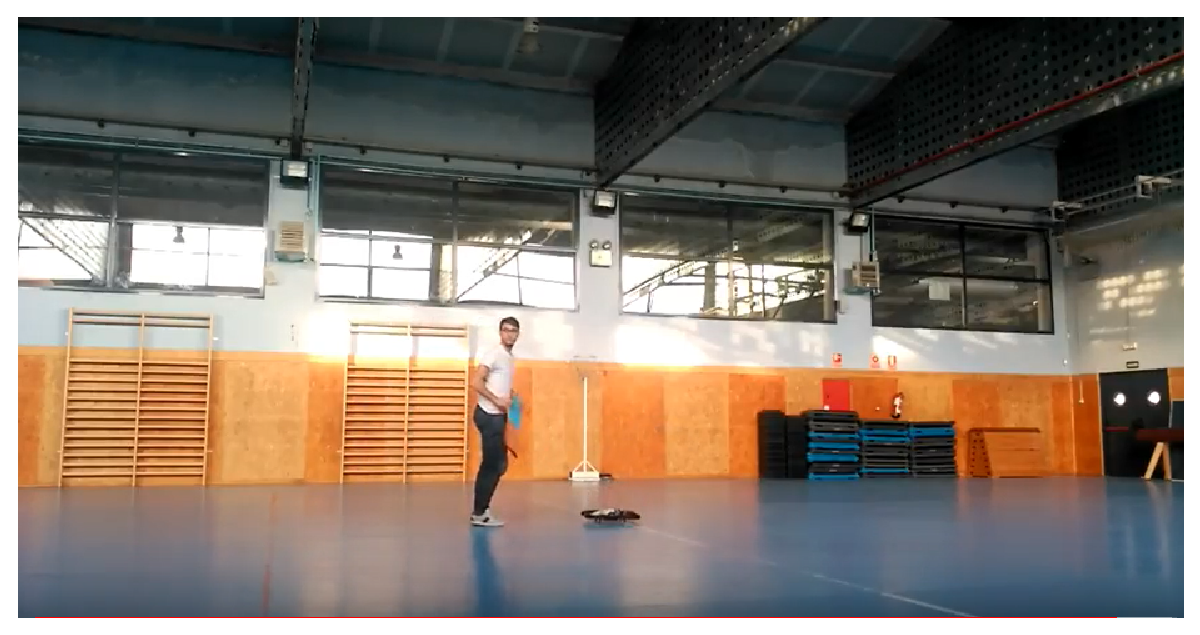
\includegraphics[width=0.3\textwidth]{imgs/balizaNaranja3.eps}}
 \caption{Aterrizaje}
 \label{f:Test 1}
\end{figure}

\hspace{1 cm} Despues de esta prueba en el mismo lugar, decidimos probar el algoritmo de busqueda, sin encontrar la baliza, solo ver que una vez que despegaba se desplazaba realizando una espiral, prueba que quedo grabada y tambi\'en se realizo con \'exito.

\hspace{1 cm} Ya teniendo el algoritmo de busqueda y un primer filtro de color, las pruebas se centraron en que el dron consiguiera centrarse sobre una baliza tras despegar. En un principio fue complicado, pues el dron que se ten\'ia para realizar las pruebas al despegar, en los dos segundos que no teniamos control sobre el, en lugar de subir verticalmente lo hac\'ia en diagonal hacia atras, lo que nos llevo a comprobar que distancia recorria en este tiempo para poder jugar con ella, colocando el dron unos metros delante de la baliza, para que en el momento que se tomaba el control se situara sobre esta. Los primeros controles no eran muy fluidos, pues el algoritmo que hab\'ia para detectar el color e indicar sobre el GUI eran un poco pesados, y a�adiendo a eso que solo se ten\'ia un control progresivo, oscilaba mucho,  llegando un momento que perdia la baliza. Debido a esto se mejoro sobre todo el control, aunque tambi\'en el algoritmo, utilizando mas funciones de OpenCV, por ejemplo. Con todo esto, el dron se manten\'ia sobre la baliza aunque continuaba oscilando mas de lo que debiera. Poco a poco se fue ajustando para que la oscilacion fuera m\'inima.

\hspace{1 cm} Como con un color ya teniamos grandes avances, se volvio a trabajar sobre la baliza real, lo que nos llevo a ajustar de nuevo un poco la parte del filtro de color y la informaci\'on que se enviaba debido a este, pues en cada prueba pr\'acticamente habia que modificar parte del pre-procesado debido a las condiciones del lugar. Pero una vez se vio que era algo robusto se intento trabajar de nuevo en lugares de menor tama�o, y destacar que las pruebas salieron bien, pues habiendo calculado la distancia que recorria en diagonal, al contar con esta distancia en el despegue, cuando se tomaba control del dron, este ve\'ia la baliza que se le tenia puesta, por lo tanto ejecutaba las instrucciones que se le enviaban y no se desviaba mas de lo debido. 
\hspace{1 cm} El problema de comenzar a trabajar en este entorno de trabajo fue que el suelo era de un color muy parecido al que ten\'iamos en la baliza, y por tanto se tuvieron que ajustar de nuevo los filtros de color. Decir que de nuevo se volvian a producir mas oscilaciones de las esperadas , as\'i que para evitar esto finalmente se a�adio lo llamado banda muerta, de forma que si la desviaci\'on es minima no intente centrarse sino que se quede en el sitio, y si la desviaci\'on se encuentra dentro de unos limites se corriga muy brevemente, consiguiendo asi que el dron este situado sobre cierto area, que era lo que se pretendia, aunque no sea exactamente el centro.
  \newline
\hspace{1 cm} Como se puede observar, todas estas son las pruebas realizadas con materiales reales, pero destacar que todas estas, antes de probarlas as\'i fueron realizadas en el simulador, ya que era lo mas comodo para trabajar calculando areas, centros y la utilizaci\'on de operadores morfol\'ogicos. Contar las pruebas realizadas sobre este ser\'ia repetir en cierta forma el proceso, pero si me gustar\'ia destacar la primera prueba que se hizo con el controlador PD, pues en videos vistos a posteriori se puede comprobar la diferencia de oscilaci\'on, pues en el real cuando oscilaba mucho el dron, perdia la baliza y se le mandaba la instrucci\'on de quedarse en el sitio para que pudiera aterrizar, en el simulador se ve\'ia como giraba bruscamente, perdia la baliza y volvia a su posici\'on, donde volvia a ver la baliza lo que le llevaba a girar bruscamente de nuevo, as\'i durante varias iteraciones hasta que se centraba y se paraba ese movimiento brusco. Sin embargo cuando se a�adio este controlador se veia como por el cambio de velocidad tenia un punto de frenado debido a la diferencia entre velocidades y poco a poco volvia a acelerar en una direcci\'on o frenar, segun lo requerido en ese momento. 


\end{document}


